%%
%% This is file `sample-sigconf.tex',
%% generated with the docstrip utility.
%%
%% The original source files were:
%%
%% samples.dtx  (with options: `sigconf')
%% 
%% IMPORTANT NOTICE:
%% 
%% For the copyright see the source file.
%% 
%% Any modified versions of this file must be renamed
%% with new filenames distinct from sample-sigconf.tex.
%% 
%% For distribution of the original source see the terms
%% for copying and modification in the file samples.dtx.
%% 
%% This generated file may be distributed as long as the
%% original source files, as listed above, are part of the
%% same distribution. (The sources need not necessarily be
%% in the same archive or directory.)
%%
%%
%% Commands for TeXCount
%TC:macro \cite [option:text,text]
%TC:macro \citep [option:text,text]
%TC:macro \citet [option:text,text]
%TC:envir table 0 1
%TC:envir table* 0 1
%TC:envir tabular [ignore] word
%TC:envir displaymath 0 word
%TC:envir math 0 word
%TC:envir comment 0 0
%%
%%
%% The first command in your LaTeX source must be the \documentclass command.
%\documentclass[sigconf]{acmart}
\documentclass[sigconf,review]{acmart}

\usepackage{enumitem}
\usepackage{color, colortbl}
\usepackage{ragged2e}
\usepackage{array}
\usepackage{amsmath}
\usepackage{listings}
\lstset{
	basicstyle=\ttfamily,
	frame=none,
	breaklines=true,
	numbers=left,
	xleftmargin=2.5em,
	framexleftmargin=0em,
	emphstyle=\textbf,
	float=t
}
\lstdefinestyle{yaml}{
	basicstyle=\ttfamily\small,
	emph={-, :, nsuri, ? }
}

\hyphenation{
	Ex-po-nent-ia-ted-Gra-di-ent-Re-duct-ion
	Ex-po-nent-ia-ted Gra-di-ent Re-duct-ion
	lo-ad pre-proc da-ta a-dult
	Lo-gis-tic-Re-gress-ion
}

%%
%% \BibTeX command to typeset BibTeX logo in the docs
\AtBeginDocument{%
  \providecommand\BibTeX{{%
    \normalfont B\kern-0.5em{\scshape i\kern-0.25em b}\kern-0.8em\TeX}}}

%% Rights management information.  This information is sent to you
%% when you complete the rights form.  These commands have SAMPLE
%% values in them; it is your responsibility as an author to replace
%% the commands and values with those provided to you when you
%% complete the rights form.
\setcopyright{acmcopyright}
\copyrightyear{2022}
\acmYear{2022}
\acmDOI{XXXXXXX.XXXXXXX}

%% These commands are for a PROCEEDINGS abstract or paper.
\acmConference[MODELS '22]{ACM / IEEE 25th International Conference on Model Driven Engineering Languages and Systems}{October 23--28,
  2022}{Montreal, Canada}
\acmPrice{15.00}
\acmISBN{978-1-4503-XXXX-X/22/10}


%%
%% Submission ID.
%% Use this when submitting an article to a sponsored event. You'll
%% receive a unique submission ID from the organizers
%% of the event, and this ID should be used as the parameter to this command.
%%\acmSubmissionID{123-A56-BU3}

%%
%% The majority of ACM publications use numbered citations and
%% references.  The command \citestyle{authoryear} switches to the
%% "author year" style.
%%
%% If you are preparing content for an event
%% sponsored by ACM SIGGRAPH, you must use the "author year" style of
%% citations and references.
%% Uncommenting
%% the next command will enable that style.
%%\citestyle{acmauthoryear}

%%
%% end of the preamble, start of the body of the document source.
\begin{document}

%%
%% The "title" command has an optional parameter,
%% allowing the author to define a "short title" to be used in page headers.
\title{Towards Model-based Bias Mitigation in Machine Learning}

%%
%% The "author" command and its associated commands are used to define
%% the authors and their affiliations.
%% Of note is the shared affiliation of the first two authors, and the
%% "authornote" and "authornotemark" commands
%% used to denote shared contribution to the research.
%\author{Ben Trovato}
%\authornote{Both authors contributed equally to this research.}
%\email{trovato@corporation.com}
%\orcid{1234-5678-9012}
%\author{G.K.M. Tobin}
%\authornotemark[1]
%\email{webmaster@marysville-ohio.com}
%\affiliation{%
%  \institution{Institute for Clarity in Documentation}
%  \streetaddress{P.O. Box 1212}
%  \city{Dublin}
%  \state{Ohio}
%  \country{USA}
%  \postcode{43017-6221}
%}
%
%\author{Lars Th{\o}rv{\"a}ld}
%\affiliation{%
%  \institution{The Th{\o}rv{\"a}ld Group}
%  \streetaddress{1 Th{\o}rv{\"a}ld Circle}
%  \city{Hekla}
%  \country{Iceland}}
%\email{larst@affiliation.org}
%
%\author{Valerie B\'eranger}
%\affiliation{%
%  \institution{Inria Paris-Rocquencourt}
%  \city{Rocquencourt}
%  \country{France}
%}
%
%\author{Aparna Patel}
%\affiliation{%
% \institution{Rajiv Gandhi University}
% \streetaddress{Rono-Hills}
% \city{Doimukh}
% \state{Arunachal Pradesh}
% \country{India}}
%
%\author{Huifen Chan}
%\affiliation{%
%  \institution{Tsinghua University}
%  \streetaddress{30 Shuangqing Rd}
%  \city{Haidian Qu}
%  \state{Beijing Shi}
%  \country{China}}
%
%\author{Charles Palmer}
%\affiliation{%
%  \institution{Palmer Research Laboratories}
%  \streetaddress{8600 Datapoint Drive}
%  \city{San Antonio}
%  \state{Texas}
%  \country{USA}
%  \postcode{78229}}
%\email{cpalmer@prl.com}
%
%\author{John Smith}
%\affiliation{%
%  \institution{The Th{\o}rv{\"a}ld Group}
%  \streetaddress{1 Th{\o}rv{\"a}ld Circle}
%  \city{Hekla}
%  \country{Iceland}}
%\email{jsmith@affiliation.org}
%
%\author{Julius P. Kumquat}
%\affiliation{%
%  \institution{The Kumquat Consortium}
%  \city{New York}
%  \country{USA}}
%\email{jpkumquat@consortium.net}

\author{Alfa Yohannis}
\affiliation{%
	  \institution{University of York}
	  \city{York}
	  \country{United Kingdom}}
\email{alfa.yohannis@york.ac.uk}

\author{Dimitris Kolovos}
\affiliation{%
	\institution{University of York}
	\city{York}
	\country{United Kingdom}}
\email{dimitris.kolovos@york.ac.uk}

%%
%% By default, the full list of authors will be used in the page
%% headers. Often, this list is too long, and will overlap
%% other information printed in the page headers. This command allows
%% the author to define a more concise list
%% of authors' names for this purpose.
\renewcommand{\shortauthors}{Yohannis and Kolovos}

%%
%% The abstract is a short summary of the work to be presented in the
%% article.
\begin{abstract}
Models produced by machine learning are not guaranteed free from bias, particularly when trained and tested with data produced in discriminatory environments. The bias can be unethically acceptable, especially when the data contains sensitive attributes, such as sex, race, age, etc. Some approaches have contributed to mitigating such biases by providing bias metrics and mitigation algorithms. The challenge is users have to implement their code in general/statistical programming languages which can be demanding for users with little programming and fairness in machine learning experience. FairML provides a model-based approach to improve the productivity of bias measurement and mitigation by raising up their abstraction and automatically generating their implementation code. Our evaluation shows that FairML requires fewer lines of code to produce similar measurement values, with $pm$ 0.1 tolerance, to the ones produced by the baseline code.
\end{abstract}

%%
%% The code below is generated by the tool at http://dl.acm.org/ccs.cfm.
%% Please copy and paste the code instead of the example below.
%%
\begin{CCSXML}
	<ccs2012>
	<concept>
	<concept_id>10011007.10011006.10011041.10011047</concept_id>
	<concept_desc>Software and its engineering~Source code generation</concept_desc>
	<concept_significance>500</concept_significance>
	</concept>
	<concept>
	<concept_id>10003752.10010070.10010071</concept_id>
	<concept_desc>Theory of computation~Machine learning theory</concept_desc>
	<concept_significance>300</concept_significance>
	</concept>
	<concept>
	<concept_id>10010405.10010455</concept_id>
	<concept_desc>Applied computing~Law, social and behavioral sciences</concept_desc>
	<concept_significance>500</concept_significance>
	</concept>
	</ccs2012>
\end{CCSXML}

\ccsdesc[500]{Software and its engineering~Source code generation}
\ccsdesc[300]{Theory of computation~Machine learning theory}
\ccsdesc[500]{Applied computing~Law, social and behavioral sciences}

%%
%% Keywords. The author(s) should pick words that accurately describe
%% the work being presented. Separate the keywords with commas.
\keywords{Model-Driven Engineering, Generative Programming, Bias Mitigation, Bias Metrics, Machine Learning}

%% A "teaser" image appears between the author and affiliation
%% information and the body of the document, and typically spans the
%% page.
%\begin{teaserfigure}
%  \includegraphics[width=\textwidth]{sampleteaser}
%  \caption{Seattle Mariners at Spring Training, 2010.}
%  \Description{Enjoying the baseball game from the third-base
%  seats. Ichiro Suzuki preparing to bat.}
%  \label{fig:teaser}
%\end{teaserfigure}

%%
%% This command processes the author and affiliation and title
%% information and builds the first part of the formatted document.
\maketitle

\section{Introduction}
\label{sec:introduction}
The use of machine learning is pervasive nowadays, from personal daily activities, such as face recognition for authentication and voice processing when talking to smart assistants (e.g., Alexa, Siri), to performing sensitive, ethical tasks, such as predicting criminals and classifying profiles for loans. While machine learning does bring efficiency, models produced by machine learning are not guaranteed free from bias, particularly when trained and tested with data produced in discriminatory environments. The bias can be unethically acceptable, particularly when it touches sensitive attributes, such as sex, race, age, etc., and cause unfairness. 

In 2016, an algorithm for predicting recidivism was found produced high false negative rate for white people and high false positive rate for black people \cite{angwin2016machine}. Some commercial face recognition services were also found having significant lower accuracy on darker-skin females \cite{buolamwini2018gender}. Moreover, A job platform was found to rank qualified female candidates far lower than qualified male candidates even though they have similar properties \cite{lahoti2019ifair}. These are some of many other instances that show biases in machine learning can promote unfairness. 

Some approaches have contributed to the mitigation of such biases by providing bias metrics and debiasing algorithms (more in Sections \ref{sec:bias_metrics} and \ref{sec:bias_mitigation}). 
These metrics and algorithms have been implemented by different toolkits.
However, they come with different methodological approaches and capabilities which demand users to understand them before they can decide which toolkits are best for specific scenarios~\cite{lee2021landscape}.  

Data scientists usually work using their intuitions to narrow down the number of combinations of algorithms, parameters, and other factors in order to find the best models for given goals, datasets, and domains \cite{muller2016introduction}. After that, with lots of experimentation and trial and error \cite{byrne2017development}, they have to go through all the narrowed combinations and test the produced models to identify which models are the best. Moreover, regardless of the availability of machine learning libraries, data scientists have to craft the search process from scratch in general/statistical programming languages (e.g, Python, R).

Model-Driven Sofware Development (MDSE) leverage the abstraction of software development by hiding technical details of implementation that can be automated \cite{brambilla2017model}. Thus, users can focus on important aspects through the use of simpler modelling languages, and the target implementation can be automatically generated, which in turn improve productivity \cite{volter2013model}. The use of MDSE would benefit data scientists since it allows them to search for the best bias mitigation methods for given cases at a higher abstraction level. They also do not have to code the implementation of the search process in general/statistical programming languages since it can be automatically generated and then fine tuned later on. 

FairML is a tool that implements the MDSE approach to model and automate bias measurement and mitigation in machine learning. 
\begin{enumerate}
	\item FairML raises the abstraction of bias measurement and mitigation so that users can configure their bias mitigation model in YAML (YAML Ain’t Markup Language), a human-friendly declarative language \cite{evans2017yaml}, without having to code in general/statistical programming languages.
	\item FairML supports a certain degree of expressiveness, allowing users to experiment with different kinds of bias metrics, bias mitigation algorithms, datasets, classifiers, and their parameters to find the best combinations that reduce biases but with acceptable accuracy.
	\item It automatically generates Python and Jupyter Notebook files which users can execute to run measure and mitigate biases on given datasets. All generated files are modifiable and extensible for fine-tuning and further development.
\end{enumerate}

This paper is structured as follow. First, we discuss fairness in machine Learning in Section \ref{sec:bias_in_machine_learning}. The section covers the definitions of some related terms, factual examples, bias metrics, and bias mitigation. In Section \ref{sec:model_based_bias_mitigation}, we presents an overview of are development as well as our approach in implementing the techniques from the field to automate bias mitigation. Section \ref{sec:example} presents how users use an existing toolkit in expressing a solution to mitigate bias in classification. We also demonstrate how FairML expresses the solution in more readable, shorter lines and is able to automatically produce generated code with the same correctness compared to the manually crafted ones. In section \ref{sec:evaluation}, we evaluate FairML on expressiveness, correctness, generation time, and execution time and use existing code of a bias mitigation toolkit as the benchmark. Section \ref{sec:result_and_discussion} presents and discusses the result of the evaluation. We also reflect on some lessons we learned during the research and development of FairML in Section \ref{sec:lessons_learned}. Finally, Section \ref{sec:conclusions_and_future_work} presents the conclusions and future work of this research.

\section{Bias in Machine Learning}
\label{sec:bias_in_machine_learning}
In this section, we briefly discuss fairness in machine learning which covers the definitions of some related terms, factual examples, bias metrics, and bias mitigation.

\subsection{Definitions and Examples}
\label{sec:definitions_and_examples}

Fairness in defined as ``the absence of any prejudice or favouritism toward an individual or
group based on their inherent or acquired characteristics'' \cite{mehrabi2021survey}.
The absence of fairness can be caused by bias which is a systematic error or distortion from the true state of affairs due to flaws in data collection and processing, study design, analysis, and interpretation \cite{oxford2022bias}. 
The unfairness happens when biases put privileged groups at the advantaged position against unprivileged groups \cite{bellamy2018ai}. 
Bias can also be caused by negative discrimination if the distinction made is due to intentional or unintentional stereotyping and prejudice based on sensitive attributes (race, age, sex, etc.) \cite{mehrabi2021survey,chen2019fairness}. 

For examples, in 2006, it has been found that COMPAS, the algorithm used for recidivism prediction produces much higher false positive rate for black people than white people \cite{angwin2016machine}. Another example is XING, a job platform similar to LinkedIn, was found to rank less qualified male candidates higher than more qualified female candidates \cite{lahoti2019ifair}. The paper states that fairness between female and male groups has been achieved, but group fairness did not necessarily indicate fairness for individuals. Moreover, publicly available commercial face recognition online services provided by Microsoft, Face++, and IBM respectively are found to suffer from achieving much lower accuracy on females with darker skin color \cite{buolamwini2018gender}. There are other examples of biases in machines learning, but these three examples already demonstrate that, in practise, machine learning is not always fair, and the unfairness can bring disadvantages to certain groups. 


\subsection{Bias Metrics}
\label{sec:bias_metrics}

\begin{figure*}[h]
	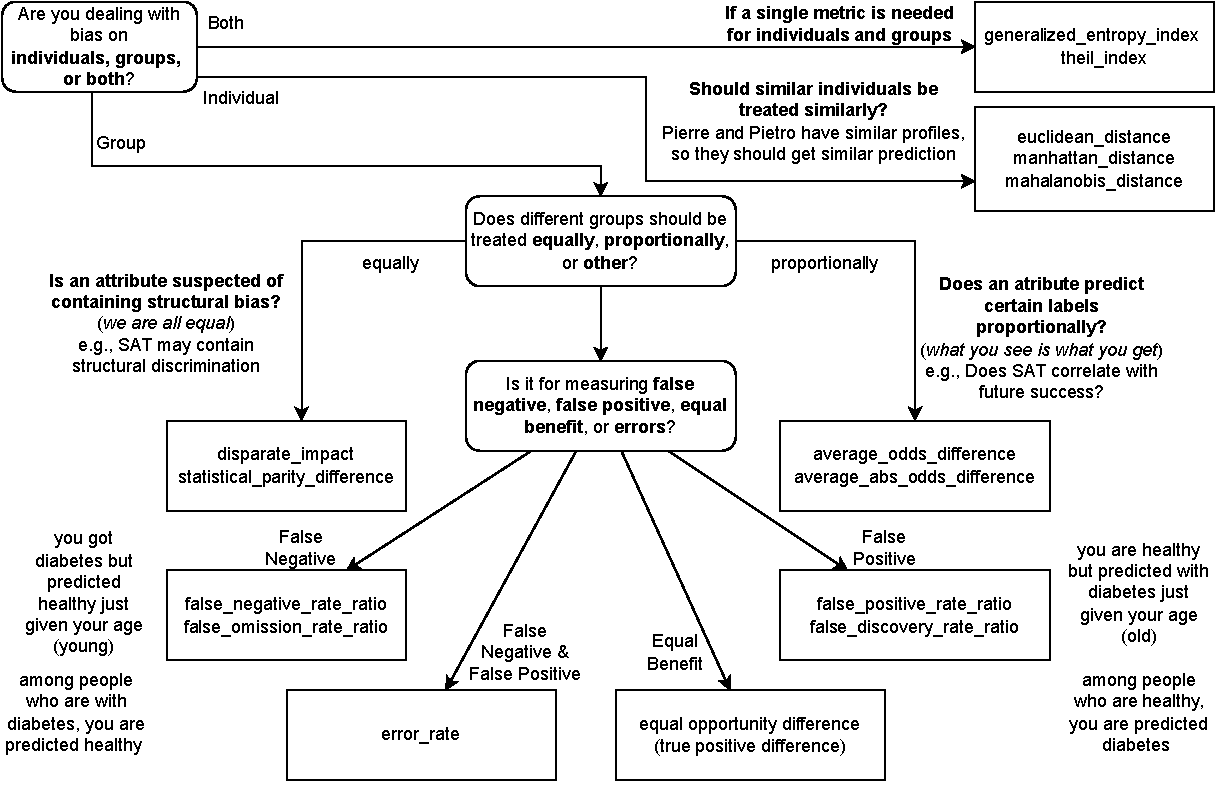
\includegraphics[width=\linewidth]{figures/wizard-metric}
	\caption{The decision tree to automatically select the most appropriate bias metrics for particular situations.}
	\label{fig:wizard-metric}
\end{figure*}

Some metrics have been developed to detect and measure biases in machine learning. Each metric has its own way to calculate biases and therefore is more preferable than others in particular situations. IBM AI Fairness 360\footnote{\url{https://aif360.mybluemix.net/resources\#guidance}} \cite{mahoney2020ai} and Aequitas\footnote{\url{http://aequitas.dssg.io/static/images/metrictree.png}} have provided guidances for the selection. If a bias measurement requires metrics that encompasses group and individual fairness then Theil Index \cite{conceicao2000theyoung,bellamy2018ai} and Generalized Entropy Index \cite{speicher2018unified} are preferable. Theil Index is the generalized entropy index  but with alpha equals to 1. They can be used as a unified metric to measures the inequality in benefit allocation for groups and individuals. Lower scores reflect strong fairness while the higher ones show the opposite. Perfect fairness is indicated by a value of 0. 

If a bias detection aims only to measure individual fairness then Euclidean Distance, Manhattan Distance, and Mahalanobis Distance are the options. These metrics are used to measure the distance of the same individual in the original and debiased datasets \cite{bellamy2018ai}. Applying bias mitigation in preprocessing can deliver group fairness but with the risk sacrificing individual fairness. The approach in \cite{calmon2017optimized} aims for group fairness but uses these metrics as constraints to limit the distortion of its bias mitigation. 

There are two main world views for group fairness: equal and proportional fairness \cite{mahoney2020ai,bellamy2018ai}. Equal fairness means under-represented groups should have a similar chance as the rest regarding prediction results and usually is applied to systems perceived to have structural discrimination. For example, A-level, SAT, or other national exams are suspected contain structural discrimination.

The first metric is Statistical parity Difference \cite{dwork2012fairness,bellamy2018ai}. The metric computed as the difference of probabilities of being labelled favourable between the privileged and unprivileged groups. The ideal value of the metric is 1.
\begin{equation} \label{eq:1}
	SPD = Pr(\hat{Y} = 1 | D = \text{unprivileged})
	- Pr(\hat{Y} = 1 | D = \text{privileged})
\end{equation}
The ideal value of the metric is 0. A negative value implies that the labelling favours the privileged group while a positive value implies the opposite.

Another metric is Disparate Impact \cite{feldman2015disparate,bellamy2018ai} which is computed as the ratio of probabilities of being labelled favourable between the unprivileged and privileged groups.
\begin{equation}
	DI = \frac{Pr(\hat{Y} = 1 | D = \text{unprivileged})}
	{Pr(\hat{Y} = 1 | D = \text{privileged})}
\end{equation}
The ideal value of this metric is 1.0. A value $<$ 1 indicates that the labelling advantages the privileged group and a value $>$ 1 disadvantage the unprivileged group.


In contrast, proportional fairness, a.k.a. what you see is what you get (WYSIWYG),  perceive that certain features correlate with labels and therefore the features can be used for prediction. For example, the scores of A-level, SAT, or other national exams correlate with incomes in the future.

Average Odds Difference \cite{bellamy2018ai} is a metric that computes bias as the average difference of false positive rate ($FPR = FP/N$, false positives / all negatives) and true positive rate ($TPR = TP/P$, true positives / positives) between unprivileged and privileged groups.
\begin{equation}
	\begin{aligned}
		AOD = \tfrac{1}{2}* ((FPR_{D = \text{unprivileged}} - FPR_{D = \text{privileged}}) +\\
		(TPR_{D = \text{unprivileged}} - TPR_{D = \text{privileged}}))
	\end{aligned}
\end{equation}
The ideal value of the metric is 0. A negative value indicates the privileged group is more favourable than the unprivileged group while a positive value indicates the opposite. 




Equal Opportunity Difference \cite{bellamy2018ai} is a metric that calculates bias as the difference of true positive rates between the unprivileged and the privileged groups. 
\begin{equation}
	EOD = TPR_{D = \text{unprivileged}} - TPR_{D = \text{privileged}}	
\end{equation}
The true positive rate is the ratio of true positives to the total number of all positive outcomes ($TPR=TP/P$) for a given group. The ideal value is 0, and a negative value indicates higher preference to the privileged group while a positive one is the opposite.



\begin{figure*}
	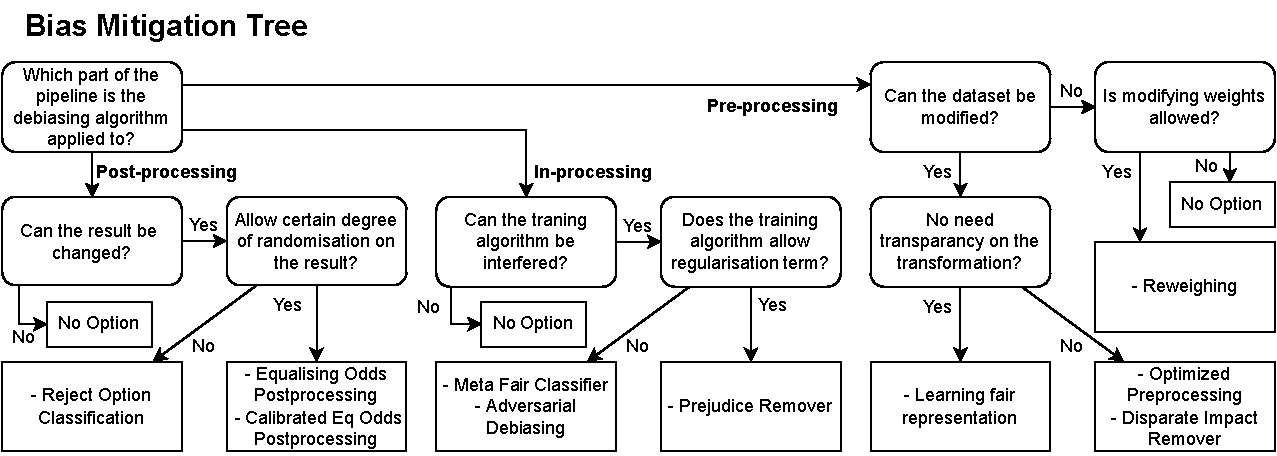
\includegraphics[width=\linewidth]{figures/wizard-debiasing}
	\caption{The decision tree to automatically select the most appropriate debiasing algorithms based on the answers to the wizard's questions.}
	\label{fig:wizard-debiasing}
\end{figure*}

\subsection{Bias Mitigation}
\label{sec:bias_mitigation}

Debiasing algorithms have been developed to reduce biases in machine learning, and they can be categorised based on the stages where they are applied in machine learning pipelines: pre-processing, in-processing, and post-processing. 

In preprocessing, \textbf{Optimized Preprocessing} \cite{calmon2017optimized} and \textbf{Disparate Impact Remover} \cite{feldman2015disparate} reduce biases by modifying the values of features of a dataset, implying that the dataset should be modifiable. 
Optimized Preprocessing learns a probabilistic transformation that modify the labels and features of a dataset but with objectives and constraints on individual distortion, data fidelity, and group fairness.
Disparate impact remover alters the values of features to increase the fairness of groups while preserving rank-ordering within groups.
\textbf{Learning Fair Representation} (LFR) \cite{zemel2013lfr} preprocesses a dataset by encoding data into a latent space and obfuscates the values of protected attributes.
\textbf{Reweighing} \cite{kamiran2011reweighing} does not alter the values of features but works by altering only the weight of each label/prediction to gain fairness. All of these debiasing algorithms aim to ensure fairness before classification.

In inprocessing, \textbf{Prejudice Remover} \cite{kamishima2012prejudice} adds a discrimination-aware regularization term to the learning objective.
\textbf{Meta Fair Classification} takes the fairness metric as part of the input and returns a classifier optimized with respect to that fairness metric.
\textbf{Grid Search Reduction} is an in-processing technique that can be used for fair classification or fair regression. For classification it reduces fair classification to a sequence of cost-sensitive classification problems, returning the deterministic classifier with the lowest empirical error subject to fair classification constraints among the candidates searched. For regression it uses the same priniciple to return a deterministic regressor with the lowest empirical error subject to the constraint of bounded group loss.
\textbf{Gerryfair Classification} is an algorithm for learning classifiers that are fair with respect to rich subgroups. Rich subgroups are defined by (linear) functions over the sensitive attributes, and fairness notions are statistical: false positive, false negative, and statistical parity rates. This implementation uses a max of two regressions as a cost-sensitive classification oracle, and supports linear regression, support vector machines, decision trees, and kernel regression. 
\textbf{Exponentiated Gradient Reduction} is an in-processing technique that reduces fair classification to a sequence of cost-sensitive classification problems, returning a randomized classifier with the lowest empirical error subject to fair classification constraints.
\textbf{Adversarial Debiasing} is an in-processing technique that learns a classifier to maximize prediction accuracy and simultaneously reduce an adversary's ability to determine the protected attribute from the predictions. This approach leads to a fair classifier as the predictions cannot carry any group discrimination information that the adversary can exploit.
Among in-processing algorithms, the prejudice remover is limited to learning algorithms that allow for regularization terms whereas the adversarial debiasing algorithm allows for a more general set of learning algorithms, and may be preferred for that reason.


%Adversarial Debiasing,   Exponentiated Gradient Reduction, 
%Gerryfair, Meta Fair Classification,
%Grid Search Reduction, Prejudice Remover, 

%Further Considerations
%Among pre-processing algorithms, reweighing only changes weights applied to training samples; it does not change any feature or label values. Therefore, it may be a preferred option in case the application does not allow for value changes. Disparate impact remover and optimized pre-processing yield modified datasets in the same space as the input training data, whereas LFR’s pre-processed dataset is in a latent space.  If the application requires transparency on the transformation, then disparate impact remover and optimized pre-processing may be preferred options. Moreover, optimized pre-processing addresses both group fairness and individual fairness.
%


%The current AIF360 implementations of some algorithms take arguments on which fairness metric to optimize (e.g. optimized pre-processing and reject option) and some do not (e.g. disparate impact remover and equalized odds post-processing), which may imply better and worse performance by some algorithms with respect to some metrics.  The result of improving one fairness on other fairness metrics is complicated [7].


In postprocessing, \textbf{Reject Option Classification} \cite{kamiran2012reject} gives favourable outcomes to unprivileged groups but also does the opposite to privileged groups in a confidence band around the decision boundary with the highest uncertainty.
\textbf{Equalised Odds Postprocessing} \cite{hardt2016equal,pleiss2017equal} solves a linear program to find probabilities with which to change output labels to optimise equalized odds.
\textbf{Calibrated Equalised Odds Postprocessing} \cite{pleiss2017equal} optimises over calibrated classifier score outputs to find probabilities with which to change output labels with an equalised odds
objective. 
Both equalized odds algorithms have a randomised component while the reject option algorithm is deterministic.


\section{Model-based Bias Mitigation}
\label{sec:model_based_bias_mitigation}

In this section, we present an overview of Model-driven Software Development, and then we proceed with our domain analysis. The analysis is used as the base for the design of FairML. 


\subsection{Model-driven Software Development}
\label{sec:model_based_software_development}
Model-Driven Sofware Development (MDSD) is a development paradigm in software engineering that it uses models as the main artefacts to drive the processes of software development. The models are used as bases or references to (semi)automatically generate the target software \cite{brambilla2017model}. 

MDSE aims for a productive environment by speeding up development through artefact generation and managing complexity by raising up abstraction level in the form of simpler modelling languages, such as domain-specific Languages (DSLs) \cite{volter2013model}. 

%\begin{table*}[]
%	\centering
%	\caption{Toolkits for bias mitigation in machine learning.}
%	\label{tab:bias-mitigation-toolkits}
%	\begin{tabular}{p{.15\textwidth}p{.39\textwidth}p{.39\textwidth}}
%		\hline
%		\multicolumn{1}{c}{\textbf{Toolkit}}                                   & \multicolumn{1}{c}{\textbf{Website}}                                                                                                  & \multicolumn{1}{c}{\textbf{Repository}}                                                                                     \\ \hline
%		Fairlearn                                                              & \url{https://fairlearn.org}                                                                                                                 & \url{https://github.com/fairlearn/fairlearn}                                                                                      \\
%		Google What-If                                                         & \url{https://pair-code.github.io/what-if-tool}                                                                                              & \url{https://github.com/pair-code/what-if-tool}                                                                                   \\
%		Scikit-fairness, Scikit-lego & \url{https://scikit-fairness.netlify.app}, \url{https://scikit-lego.readthedocs.io/en/latest/index.html} & \url{https://github.com/koaning/scikit-fairness},  \url{https://github.com/koaning/scikit-lego} \\
%		IBM AI Fairness 360                                                    & \url{https://aif360.mybluemix.net}                                                                                                          & \url{https://github.com/Trusted-AI/AIF360}                                                                                        \\ \hline
%	\end{tabular}
%\end{table*}

\subsection{Toolkit Selection}
\label{sec:toolkit_selection}
MDSE relies heavily on code generation to produce running code. This means it also requires existing tools or libraries to be used in the generated code. Therefore, we need to identify existing tools or libraries that can execute bias mitigation in the generated code. 

Lee et al. \cite{lee2021landscape} analysed the landscape of open source toolkits in algorithmic ethics, particularly for fair machine learning. With criteria that the toolkit 1) should be open source, 2) is likely to be used by practitioners, and 3) is implementing fairness-related methodology and through a focus group discussion of data scientists, they selected 6 best toolkits for fair machine learning and used them further in their analysis. The toolkits are Aequitas\cite{saleiro2019aequitas}, Google What-If\cite{googlewhatif2020}, Scikit-fairnet/scikit-lego \cite{scikitfairness2022,scikitlego2022}, Fairlearn\cite{bird2020fairlearn}, and IBM AI Fairness 360 \cite{bellamy2018ai}.  

From these the six toolkits, we evaluate them again to examine if they are applicable to be integrated into our model-based approach. The selected toolkits would be used in the generated code to implement bias mitigation. The main criteria for the selection are 1) it should be open source, 2) it should support bias mitigation, 3) it provides Application Programming Interface (API) to be programmable and integrated into model-based approach, and 4) it supports various bias measurements and mitigation algorithms to enable users to find the best bias mitigation strategies. 

The first criterion is met by all of the toolkits, since they are all open source projects. We excluded Aequitas due to its inability to perform bias mitigation (second criterion); it only supports bias measurement. We also removed Google What-If since it does not have API\footnote{\url{https://groups.google.com/g/what-if-tool/c/zw4Rk5kxPIM}} to be integrated with other applications (third criterion); its customisation is limited to custom prediction function\footnote{\url{https://pair-code.github.io/what-if-tool/get-started/}}. IBM AI Fairness 360 has the most complete features -- it claims it has at least 10 state-of-the-art bias mitigation algorithms and 77 bias metrics\footnote{\url{https://aif360.mybluemix.net/}} while Fairlearn and Scikit-fairness/lego come second and third \cite{lee2021landscape}. All of them meet the fourth criteria. However, since IBM AI Fairness 360 has the most complete features, we prioritise to implement our bias mitigation implementation code using the toolkit. Also, the IBM toolkit supports Fairlearn' Grid Search Reduction\footnote{\url{https://github.com/Trusted-AI/AIF360/blob/master/aif360/algorithms/inprocessing/grid\_search\_reduction.py}} and Exponentiated Gradient Reduction\footnote{\url{https://github.com/Trusted-AI/AIF360/blob/master/aif360/algorithms/inprocessing/exponentiated\_gradient\_reduction.py}} algorithms.

%Nevertheless, we still refer to Fairlearn and Scikit-fairness/lego's code repositories and documentations to understand how bias mitigation implemented. 

%They also identified that there was a lack of consistency between the toolkits in their methodological approaches, and therefore users need to understand them at first before they can use the toolkits properly to meet goals.

\subsection{Domain Analysis}
\label{sec:domain_analysis}

In order to model bias mitigation in machine learning, important constructs and workflows of the domain should be accommodated by the model \cite{volter2013model}. Usually, interviewing the experts in the field is the common option to capture the constructs and workflows. However, this can be challenging particularly in research or development with limited resources (e.g., low fund, tight schedules, expert availability). Therefore, we opted for document analysis as documents contain information to understand the objects of interests \cite{bowen2009document}. As showcases, Poncin et al. \cite{poncin2011process} and Rogers et al. \cite{rogers2015using} analysed code repositories and existing documentation to understand software development and maintenance processes. Thus, we analyse the code repository and documentation of IBM AI Fairness 360 in order to understand its uses and implementation in mitigating bias as they reflect bias mitigation in practice. Our domain analysis aimed to identify important constructs and workflows in the examples, demos, and tutorials provided by the toolkit. The important constructs are crucial for abstraction so that users only deal with them when constructing models and therefore reducing complexity. Workflow is important to understand the order in defining and executing the construct.

%\begin{figure}
%	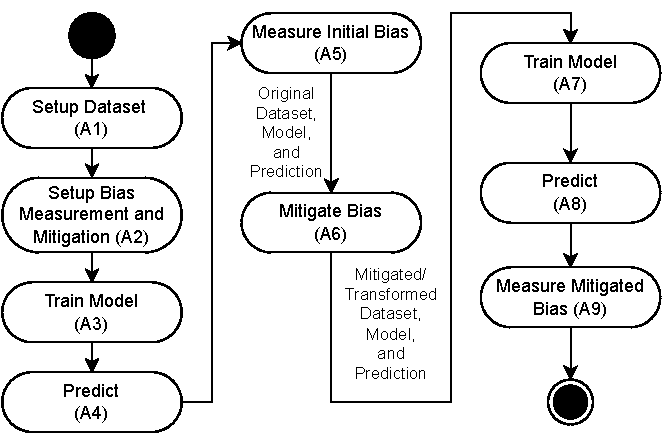
\includegraphics[width=\linewidth]{figures/workflow}
%	\caption{The workflow of bias mitigation commonly performed using the toolkits in Section \ref{sec:toolkits}.}
%	\label{fig:workflow}
%\end{figure}

Our analysis found that, in general, bias measurement and mitigation  executes the following actions. They are executed in order but certain actions can be skipped if they are not necessary. Important constructs are formatted in italic.

\begin{itemize}
\item[\textbf{A01:}] \textbf{Setup Datasets}. Bias mitigation usually starts with setting up \textit{datasets}. In the action, users define the \textit{source} of every dataset which is commonly a \textit{CSV file}. They also profile each dataset to determine which attribute is the \textit{predicted attribute} (including the \textit{favourable class} in the attribute) and the \textit{sensitive attributes} (including the \textit{privileged} and \textit{unprivileged classes} in the attributes). Using \textit{built-in datasets} provided by a toolkit is also another option. 
The \textit{training}, \textit{validation}, and \textit{test datasets} are also set here, whether they are all come from different datasets or the same dataset but is \textit{split} in different ratios. They also select the \textit{bias metrics} and \textit{mitigation algorithms} that will be applied to datasets, \textit{models}, and \textit{prediction}. 

\item[\textbf{A02:}] \textbf{Measure Original Biases Before Prediction}. In this action, users measure the original biases of the datasets in different metrics, such as accuracy, mean difference, etc. The results are used as benchmarks later when comparing them with the measurement results after prediction or applying bias mitigation algorithms.  

\item[\textbf{A03:}] \textbf{Train and Predict}. This action trains models, usually using the train datasets defined in Action A01. The training can extend to validation for tuning hyper-parameters to obtain the best parameters for the models. After that, users to make prediction
using the test dataset defined in Action A01. This action can be skipped if prediction is not required. For example, only biases in datasets are measured and mitigated.

\item[\textbf{A04:}] \textbf{Measure Original Biases After Prediction}. 
In this action, users measure the original accuracy and biases of the datasets, models, and prediction used in the preceding actions. The results are used as benchmarks later when comparing them against the results after bias mitigation. This action is skipped if Action A03 is also skipped.

\item[\textbf{A05:}] \textbf{Mitigate Bias}
In this action, users choose which debiasing algorithms they want to use: pre-processing, in-processing, or post-processing. Validation is also performed for tuning hyper-parameters to obtain the best parameters for the debiasing algorithms.
\begin{itemize}
	\item[a.] \textbf{Pre-processing}. Users apply debiasing algorithms to the copies of the original datasets. The transformed, debiased datasets are then used to train new models.
	\item[b.] \textbf{In-processing}. Users apply debiasing algorithms to regulate the selected classifiers. Usually the selected classifiers are the same as the ones in Action A03. The debiasing algorithms are then used to make new predictions.
	\item[c.] \textbf{Post-processing}. Users apply debiasing algorithms to the prediction results after predicting using the models in Action A03. 
\end{itemize}

\item[\textbf{A06:}] \textbf{Measure Biases After Debiasing}. In this action, users measure accuracies and biases after applying debiasing algorithms in Action A05 using the test datasets. 

\item[\textbf{A07:}] \textbf{Conclude}. In this action, the measurement results after debiasing are compared against the original measurement results obtained in Actions A02 and A04. Users then analyse the results to find the best combinations of datasets, classifiers, and debiasing algorithms with biases and accuracy that fit with their purposes. The comparisons can be presented in numbers, tables, and charts to facilitate users to analyse the effects of the datasets, classifiers, and debiasing algorithms. 
\end{itemize}

\subsection{Metamodel}
\label{sec:metamodel}
Figure \ref{fig:metamodel} shows a simplified metamodel of FairML. The \texttt{FairML} class represents a project of bias mitigation in machine learning. It can contains one or more datasets and bias mitigations. 

The \texttt{Dataset} class defines the datasets. In the class, we specify a dataset's name, predicted attribute, protected attributes, the split's ratio between train, test, and validation, as well as the path of its CSV file. We can also a dataset from the built-in IBM AI Fairness 360's datasets by specifying it using the \texttt{datasetModule} attribute.

The \texttt{BiasMitigation} class specifies the bias mitigations that the FairML project executes. The class contains three other significant classes: \texttt{TrainingMethod}, \texttt{MitigationMethod}, and \texttt{BiasMetric}. All of them are derived from the \texttt{\textit{Operation}} abstract class since they are executable and can have parameters and return certain results. The \texttt{TrainingMethod} class is used to define the algorithms for classification and prediction, while the \texttt{MitigationMethod} class specifies algorithms for bias mitigation. \texttt{BiasMetric} class determines the metrics to be used to measure biases. 

\begin{figure}
	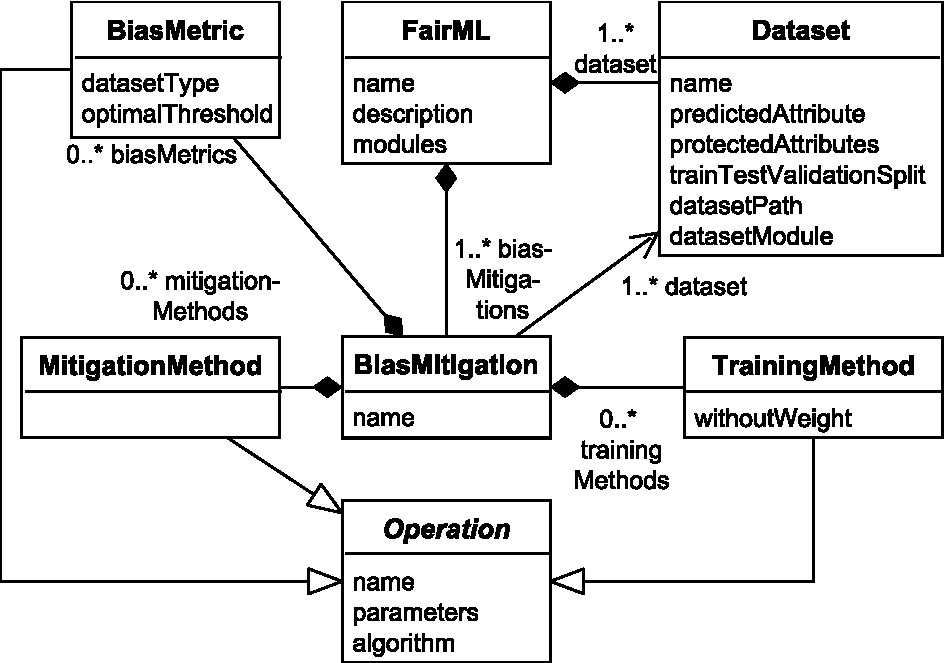
\includegraphics[width=\linewidth]{figures/metamodel}
	\caption{The Metamodel of FairML.}
	\label{fig:metamodel}
\end{figure}

\subsection{Generation}
\label{sec:generation}

Figure \ref{fig:transformation} depicts the the transformation applied by FairML to transform a bias mitigation model into Python and Jupyter Notebook files. Users only need to define their bias mitigation models in Flexmi\footnote{\url{https://www.eclipse.org/epsilon/doc/flexmi}} \cite{dimitris2016flexmi}. The model then is transformed by Epsilon Generation Language (EGL) \cite{rose2008egl} engine into Python code. The transformation itself follows the FairML's EGX/EGL\footnote{\url{https://www.eclipse.org/epsilon/doc/egl/}} rules and conforms to the defined FairML's metamodel in Ecore \cite{steinberg2009emf}.  

The generated Python files are then transformed into Jupyter notebook files using P2J\footnote{\url{https://pypi.org/project/p2j/}} engine.

\begin{figure}
	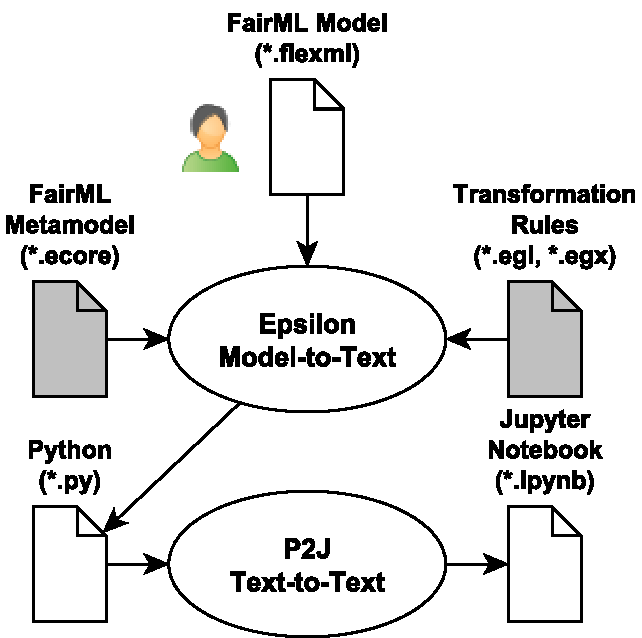
\includegraphics[width=\linewidth]{figures/transformation}
	\caption{Model-to-text transformation in fairML.}
	\label{fig:transformation}
\end{figure}



\subsection{FairML Example}
\label{sec:fairml_example}
Listing \ref{lst:fairml_model} shows a FairML model, that conforms to the metamodel in Figure\ref{fig:metamodel}, expressed in YAML. The model is the FairML version of 
IBM AI Fairness 360's Exponentiated Gradient Reduction\footnote{\url{https://github.com/Trusted-AI/AIF360/blob/master/examples/demo_exponentiated_gradient_reduction.ipynb.}} demo. The original example has a total 93 lines, excluding commented and empty lines, which is almost three times to the lines of code expressed in the listing.

The model has a name and description, \texttt{Demo} and \texttt{Debiasing using EGR} respectively, as well as adding some Python modules to be used in its components (lines 1-6). The \texttt{modules} feature is for adding additional modules that are not automatically loaded in the generated code. In the Listing, we add \texttt{load\_preproc\_data\_adult} module that is used in the \texttt{dataset} component.

The model has one dataset and one bias mitigation. The dataset is named \texttt{Adult} and is loaded from a preprocessed adult dataset provided by IBM AI Fairness 360 using \texttt{load\_preproc\_data\_adult} function. We also set \texttt{sex} as its protected attribute and split it to train, test, and validation with ratios 7:3:0 (lines 8-13). 

Lines 16-36 defines the definition of the bias mitigation executed in the \texttt{Demo} model. The bias mitigation is named \texttt{Exponentiated Gradient Reduction} and use the \texttt{Adult} dataset defined at lines 9-13 as its \texttt{dataset}. 

The bias mitigation uses three different metrics to analyse the trade-off between accuracy and fairness (mean difference, average odds difference) (lines 29-34) when the prediction uses Logistic Regression classifier only without debiasing (lines 20-22) and when the prediction is debiased using Exponentiated Gradient Reduction (lines 24-27). The former only uses one parameter; \texttt{'lbfgs'} is set as the \texttt{solver}, while the latter has three parameters; the same classifier is used as the \texttt{estimator}, \texttt{'EqualizedOdds'} is used as the \texttt{constraint}, and the protected attributes are not dropped.

\begin{lstlisting}[firstnumber=1,style=yaml,caption={Bias mitigation using  Demo Exponentiated Gradient Reduction  expressed in YAML.},label=lst:fairml_model]
?nsuri: fairml
fairml:
- name: Demo
- description: Debiasing using EGR
- modules: 
from aif360.algorithms.preprocessing.optim_preproc_helpers.data_preproc_functions import load_preproc_data_adult

# set the dataset
- dataset:
  - name: Adult
  - datasetModule: load_preproc_data_adult
  - protectedAttributes: sex
  - trainTestValidationSplit: 7, 3

# define the bias mitigation
- biasMitigation:
- name: Exponentiated Gradient Reduction  
- dataset: Adult

- trainingMethod:
  - algorithm: LogisticRegression
  - parameters: solver='lbfgs'

- mitigationMethod:
- algorithm: ExponentiatedGradientReduction
- parameters: 
    estimator=LogisticRegression(solver='lbfgs'), constraints='EqualizedOdds', drop_prot_attr=False

- biasMetric:
  - name: accuracy
- biasMetric:
  - name: mean_difference
- biasMetric:
  - name: average_odds_difference
\end{lstlisting}


\subsection{Wizard}
\label{sec:wizard}
There are many available debiasing algorithms and bias metrics that users can select to mitigates biases in machine learning. Some of them are better than others in certain context. FairML provides a wizard feature assists users to select the most appropriate debiasing algorithms and bias metrics based on their answers to the wizard's questions. The wizard follows the guidances suggested by \cite{mahoney2020ai}, IBM AI Fairness 360\footnote{\url{https://aif360.mybluemix.net/resources\#guidance}}, and Aequitas\footnote{\url{http://aequitas.dssg.io/static/images/metrictree.png}}.




\newcolumntype{L}[1]{>{\raggedright\arraybackslash}p{#1}}
\newcolumntype{C}[1]{>{\centering\arraybackslash}p{#1}}
\newcolumntype{R}[1]{>{\raggedleft\arraybackslash}p{#1}}
\begin{table*}[]
	\caption{Part 1 of 2 -- IBM AI Fairness 360 examples and the numbers of unique datasets, classifiers, de-biasing algorithms, bias metrics, and measurement values in each example.}
	\label{tab:expressiveness1}
	\begin{tabular}{ p{1em} L{10em} R{4em} R{8em} R{9em} R{12em} R{2.5em} }
		\hline
		\multicolumn{1}{c}{\textbf{Code}} &
		\multicolumn{1}{c}{\textbf{\begin{tabular}[c]{@{}c@{}}Example/File Name\\ (*.ipynb)\end{tabular}}} &
		\multicolumn{1}{c}{\textbf{Datasets}} &
		\multicolumn{1}{c}{\textbf{Classifiers}} &
		\multicolumn{1}{c}{\textbf{\begin{tabular}[c]{@{}c@{}}Debiasing\\ Algorithms\end{tabular}}} &
		\multicolumn{1}{c}{\textbf{\begin{tabular}[c]{@{}c@{}}Bias\\Metrics\end{tabular}}} &
		\multicolumn{1}{c}{\textbf{\begin{tabular}[c]{@{}c@{}}Mea-\\sure-\\ments\end{tabular}}} \\ \hline
		E01 &
		Demo Adversarial Debiasing &
		Adult &
		N/A &
		Adversarial debiasing &
		Accuracy, Balanced accuracy, Disparate impact, Average odds, Statistical parity, Equal opportunity, Theil index &
		28 \\
		E02 &
		Demo Callibrated Eq Odd Postprocessing &
		Adult, German, Compas &
		Logistic regression &
		Calibrated eq odds postprocessing &
		Mean difference, False positive rate, False negative rate, Balanced accuracy, Equal opportunity &
		13 \\
		E03 &
		Demo Disparate Impact Remover &
		Adult &
		Logistic regression &
		Disparate impact remover &
		Disparate impact &
		11 \\
		E04 &
		Demo Exponentiated Gradient Reduction &
		Adult &
		Logistic regression &
		Exponentiated gradient reduction &
		Accuracy, Mean difference, Average odds &
		8 \\
		E05 &
		Demo Gerryfair &
		Adult &
		Linear Regression, Linear SVR, Decision Tree, Kernel Ridge &
		Gerryfair &
		Gamma disparity &
		31 \\
		E06 &
		Demo LFR &
		Adult &
		Logistic regression &
		Learning fair representation &
		Balanced accuracy, Mean difference, Disparate impact &
		5 \\
		E07 &
		Demo Lime &
		Adult &
		Logistic regression, Random forest &
		Reweighing &
		Accuracy, Balanced accuracy, Disparate impact, Average odds &
		6 \\
		E08 &
		Demo MDSS Classifier Metric &
		Compas &
		Logistic regression &
		Meta fair classifier &
		Mean difference, MDSS bias score &
		7 \\
		E09 &
		Demo Meta Classifier &
		Adult &
		N/A &
		Meta fair classifier &
		Accuracy, Balanced accuracy, Disparate impact, False discovery rate &
		13 \\
		E10 &
		Demo Optim Data Preproc &
		Adult, German, Compas &
		Logistic regression &
		Optimized preprocessing &
		Balanced accuracy, Disparate impact, Average odds, Statistical parity &
		9 \\
		E11 &
		Demo Optim Preproc Adult &
		Adult &
		N/A &
		Optimized preprocessing &
		Mean difference &
		2 \\
	 	\hline
	\end{tabular}
\end{table*}

\begin{table*}[]
	\caption{Part 2 of 2 -- IBM AI Fairness 360 examples and the numbers of unique datasets, classifiers, de-biasing algorithms, bias metrics, and measurement values in each example.}
	\label{tab:expressiveness2}
	\begin{tabular}{ p{1em} L{10em} R{4em} R{8em} R{9em} R{12em} R{2.5em} }
		\hline
		\multicolumn{1}{c}{\textbf{Code}} &
		\multicolumn{1}{c}{\textbf{\begin{tabular}[c]{@{}c@{}}Example/File Name\\ (*.ipynb)\end{tabular}}} &
		\multicolumn{1}{c}{\textbf{Datasets}} &
		\multicolumn{1}{c}{\textbf{Classifiers}} &
		\multicolumn{1}{c}{\textbf{\begin{tabular}[c]{@{}c@{}}Debiasing\\ Algorithms\end{tabular}}} &
		\multicolumn{1}{c}{\textbf{\begin{tabular}[c]{@{}c@{}}Bias\\Metrics\end{tabular}}} &
		\multicolumn{1}{c}{\textbf{\begin{tabular}[c]{@{}c@{}}Mea-\\sure-\\ments\end{tabular}}} \\ \hline
		E12 &
		Demo Reject Option Classification &
		Adult, German, Compas &
		Logistic Regression &
		Reject option classification &
		Balanced accuracy, Disparate impact, Average odds, Statistical parity, Equal opportunity, Theil index &
		26 \\
		E13 &
		Demo Reweighing Preproc &
		Adult, German, Compas &
		Logistic Regression &
		Reweighing &
		Balanced accuracy, Disparate impact, Average odds,. Statistical parity, Equal opportunity, Theil index &
		16 \\
		E14 &
		Demo Short Gerryfair Test &
		Adult &
		Linear Regression, Linear SVR, Decision Tree, Kernel Ridge &
		Gerryfair &
		Gamma disparity &
		13 \\
		E15 &
		Tutorial Credit Scoring &
		German &
		N/A &
		Reweighing &
		Mean difference &
		2 \\
		E16 &
		Tutorial Medical Expenditure &
		MEPS-Dataset19, MEPSDataset20, MEPSDataset21 &
		Random Forest, Logistic Regression &
		Reweighing, Prejudice remover &
		Balanced accuracy, Disparate impact, Average odds, Statistical parity, Equal opportunity, Theil index &
		90 \\
		E17 &
		Demo Exponentiated Gradient Reduction Sklearn &
		Adult &
		Logistic Regression &
		Grid search reduction &
		\begin{tabular}[c]{@{}r@{}}Average odds\\ Accuracy\end{tabular} &
		7 \\
		E18 &
		Demo Grid Search Reduction Classification Sklearn &
		Adult &
		Logistic Regression &
		Grid search reduction &
		Average odds, Accuracy &
		4 \\
		E19 &
		Demo Grid Search Reduction Regression Sklearn &
		Lawschool GPA &
		Linear Regression &
		Grid search reduction &
		Mean absolute error &
		7 \\
		E20 &
		Demo MDSS Classifier Metric Sklearn &
		Compas &
		Logistic Regression &
		N/A &
		MDSS bias score &
		4 \\
		E21 &
		Demo New Features &
		Adult &
		Logistic Regression &
		Reweighing meta, Adversarial debiasing, Callibrated equalized odd &
		Disparate impact, Average odds, Mean difference, Accuracy &
		6 \\ \hline
	\end{tabular}
\end{table*}

\begin{table*}[]
	\caption{Lines of code of the original examples (Ori LoC), FairML models (Model LoC), and generated code (Gen LoC).}
	\label{tab:loc}
	\begin{tabular}{clrrrrrr}
		\hline
		\multicolumn{1}{c}{\textbf{Code}} &
		\multicolumn{1}{c}{\textbf{\begin{tabular}[c]{@{}c@{}}Example/File Name \\ (*.ipynb)\end{tabular}}} &
		\multicolumn{1}{c}{\textbf{\begin{tabular}[c]{@{}c@{}}Ori\\ LoC\end{tabular}}} &
		\multicolumn{1}{c}{\textbf{\begin{tabular}[c]{@{}c@{}}Model\\ LoC\end{tabular}}} &
		\multicolumn{1}{c}{\textbf{\begin{tabular}[c]{@{}c@{}}Gen\\ LoC\end{tabular}}} &
		\multicolumn{1}{c}{\textbf{\begin{tabular}[c]{@{}c@{}}Model  LoC/\\ Ori  LoC\end{tabular}}} &
		\multicolumn{1}{c}{\textbf{\begin{tabular}[c]{@{}c@{}}Gen LoC/\\ Model LoC\end{tabular}}} &
		\multicolumn{1}{c}{\textbf{\begin{tabular}[c]{@{}c@{}}Gen LoC/\\ Ori LoC\end{tabular}}} \\ \hline
		E01 & Demo Adversarial Debiasing                        & 133 &    &     &      &      &      \\
		E02 & Demo Callibrated Eqodd Postprocessing             & 257 &    &     &      &      &      \\
		E03 & Demo Disparate Impact Remover                     & 50  & 50 & 367 & 1.00 & 7.34 & 7.34 \\
		E04 & Demo Exponentiated Gradient Reduction             & 93  & 33 & 110 & 0.35 & 3.33 & 1.18 \\
		E05 & Demo Gerryfair                                    & 90  &    &     &      &      &      \\
		E06 & Demo LFR                                          & 103 &    &     &      &      &      \\
		E07 & Demo   Lime                                       & 238 &    &     &      &      &      \\
		E08 & Demo MDSS Classifier Metric                       & 130 &    &     &      &      &      \\
		E09 & Demo Meta Classifier                              & 95  & 67 & 345 & 0.71 & 5.15 & 3.63 \\
		E10 & Demo Optim Data Preproc                           & 233 &    &     &      &      &      \\
		E11 & Demo Optim Preproc Adult                          & 35  & 30 & 85  & 0.86 & 2.83 & 2.43 \\
		E12 & Demo Reject Option Classification                 & 143 &    &     &      &      &      \\
		E13 & Demo Reweighing Preproc                           & 212 & 59 & 125 & 0.28 & 2.12 & 0.59 \\
		E14 & Demo Short Gerryfair Test                         & 52  & 50 & 176 & 0.96 & 3.52 & 3.38 \\
		E15 & Tutorial Credit Scoring                           & 30  & 25 & 84  & 0.83 & 3.36 & 2.80 \\
		E16 & Tutorial Medical Expenditure                      & 356 & 90 & 554 & 0.25 & 6.16 & 1.56 \\
		E17 & Demo Exponentiated Gradient Reduction Sklearn     & 54  &    &     &      &      &      \\
		E18 & Demo Grid Search Reduction Classification Sklearn & 52  &    &     &      &      &      \\
		E19 & Demo Grid Search Reduction Regression Sklearn     & 64  &    &     &      &      &      \\
		E20 & Demo MDSS Classifier Metric Sklearn               & 66  &    &     &      &      &      \\
		E21 & Demo New Features                                 & 82  &    &     &      &      &      \\ \hline
	\end{tabular}
\end{table*}

\begin{table*}[]
	\caption{The generation time of FairML and execution time of the original examples and generated code (seconds).}
	\label{tab:time}
	\begin{tabular}{clrrrr}
		\hline
		\textbf{Code} &
		\multicolumn{1}{c}{\textbf{\begin{tabular}[c]{@{}c@{}}Example/File Name \\ (*.ipynb)\end{tabular}}} &
		\multicolumn{1}{c}{\textbf{\begin{tabular}[c]{@{}c@{}}Generation\\ Time\end{tabular}}} &
		\multicolumn{1}{c}{\textbf{\begin{tabular}[c]{@{}c@{}}Original\\ Exec Time\end{tabular}}} &
		\multicolumn{1}{c}{\textbf{\begin{tabular}[c]{@{}c@{}}Generated\\ Exec Time\end{tabular}}} &
		\multicolumn{1}{c}{\textbf{\begin{tabular}[c]{@{}c@{}}Gen/Ori\\ Exec Time\end{tabular}}} \\ \hline
		E01 & Demo Adversarial Debiasing                        &       &        &        &      \\
		E02 & Demo Callibrated Eqodd Postprocessing             &       &        &        &      \\
		E03 & Demo Disparate Impact Remover                     & 0.186 & 20.991 & 20.23  & 0.96 \\
		E04 & Demo Exponentiated Gradient Reduction             & 0.166 & 29.927 & 30.211 & 1.01 \\
		E05 & Demo Gerryfair                                    &       &        &        &      \\
		E06 & Demo LFR                                          &       &        &        &      \\
		E07 & Demo   Lime                                       &       &        &        &      \\
		E08 & Demo MDSS Classifier Metric                       &       &        &        &      \\
		E09 & Demo Meta Classifier                              & 0.192 & 12.989 & 14.67  & 1.13 \\
		E10 & Demo Optim Data Preproc                           &       &        &        &      \\
		E11 & Demo Optim Preproc Adult                          & 0.154 & 8.044  & 15.52  & 1.93 \\
		E12 & Demo Reject Option Classification                 &       &        &        &      \\
		E13 & Demo Reweighing Preproc                           & 0.158 & 1.461  & 4.633  & 3.17 \\
		E14 & Demo Short Gerryfair Test                         & 0.164 & 3.389  & 3.875  & 1.14 \\
		E15 & Tutorial Credit Scoring                           & 0.162 & 0.017  & 0.078  & 4.59 \\
		E16 & Tutorial Medical Expenditure                      & 0.198 & 34.897 & 54.248 & 1.55 \\
		E17 & Demo Exponentiated Gradient Reduction Sklearn     &       &        &        &      \\
		E18 & Demo Grid Search Reduction Classification Sklearn &       &        &        &      \\
		E19 & Demo Grid Search Reduction Regression Sklearn     &       &        &        &      \\
		E20 & Demo MDSS Classifier Metric Sklearn               &       &        &        &      \\
		E21 & Demo New Features                                 &       &        &        &      \\ \hline
	\end{tabular}
\end{table*}

\section{Evaluation}
\label{sec:evaluation}
In this research, we also evaluated the expressiveness, correctness, productivity, and execution time of FairML. In the expressiveness evaluation, we aimed to answer this question, 
``\textit{Can FairML express the use cases of bias mitigation in the real-world?}''. For that, we used the examples provided IBM Fairness AI 360 as the baseline to justify the expressiveness of FairML. 
the toolkit comes with a number of examples (Tables \ref{tab:expressiveness1} and \ref{tab:expressiveness2}) that demonstrate 
the usecases of the toolkit in the real-world context. 
Among 22 examples that comes in version 4.0, we only used 21 of them, 
since the one that we excluded only explains the use of a class dedicated to yield bias metric explanation in JSON format. We also count the numbers of bias metrics, de-biasing algorithms, classifiers, datasets, and measurement values are there in each example to reveal its complexity. 

We compared the bias metric values measured (measurement values) in the original examples with the values measured in the generated code to evaluate the correctness of FairML's generated code. Both should produce equal values or similar values, up to 10\% tolerance, when randomness is required.  

In the productivity evaluation, 
we compared the ratio of the written vs. generated code of FairML vs.
code in the examples. 
While this metric does not always guaranteed productivity in the end due many factors, 
the number of lines written by users is significantly reduced. In the measurement, \textit{markdown}, whitespace, and commented lines were not counted.

We also measured the execution time of FairML.First, we measured the \textit{generation time} -- the time that FairML takes to completely generate the target code. Second, we compared the time taken by the generated target code against the example code to to complete their operations (\textit{generated execution time} vs. \textit{original execution time}). The evaluation was performed on a machine with Windows 10 64-bit operating system, 11th Gen Intel(R) Core(TM) i9-11900H @ 2.50GHz 8-core processors, 32.0 GB RAM DDR4, OpenJDK Runtime Environment 18.9 (build 11.0.14.1+1), and Python 3.9.7.

\section{Results and Discussion}
\label{sec:result_and_discussion}
In this section, we present and discuss the results of our FairML evaluation.

\subsection{Expressiveness and Correctness}
\label{sec:expressiveness_and_correctness}
Based on our evaluation, FairML was able to reproduce all the scenarios in all the 21 examples in Tables \ref{tab:expressiveness1} and \ref{tab:expressiveness2}. In total, all the scenarios covered 8 unique datasets (Adult, German, Compas, Lawschool GPA, MEPSDataset19, MEPSDataset20, MEPSDataset21), 6 classifiers (Logistic Regression, Linear Regression, Linear SVR, Decision Tree, Kernel Ridge, Random Forest), 13 bias mitigation algorithms (Adversarial Debiasing, Callibrated Equalising Odds, Disparate Impact Remover, Exponentiated Gradient Reduction, Gerryfair, Learning Fair Representation, Reweighing, Meta Fair Classification, Optimized Preprocessing, Reject Option Classification, Prejudice Remover, Grid Search Reduction, Reweighing Meta), and 15 bias metrics (Accuracy, Balanced Accuracy, Mean Difference a.k.a. Statistical Parity Difference, Disparate Impact, Equal Opportunity Difference, Theil Index, Gamma Disparity, Average Odds Difference, Mean Absolute Error, MDSS Bias Score, False Positive Rate, False Negative Rate, False Discovery Rate, Rrror Rate, Mean Absolute Error). In addition, FairML also supports loading data from external CSV files. All of these allows users to express their bias mitigation strategies in different combinations of datasets, classifiers, de-biasing algorithms, and bias metrics.

Regarding correctness, the values that the generated code produced were dominantly equal to the measurement values in the examples. Some of them were different with tolerance less than $\pm$ 0.1 difference. From all $N$ measurement values in Tables \ref{tab:expressiveness1} and \ref{tab:expressiveness2}, equal values comprise $N1$ values, while the tolerated values cover only $N2$ values.  


\subsection{Productivity}
\label{sec:productivity}

Table \ref{tab:loc} shows a comparison on the numbers of lines of code (LoC) between the original examples, FairML models, and generated code. It shows that \textsf{Model LoC}/\textsf{Original LoC} are equal or less than 1, indicating that users would write less code to produce the same results as in the examples (see Section \ref{sec:expressiveness_and_correctness} for correctness). Moreover, the efficiency also gets higher as the number of original LoC increases as can been seen at the examples \textsf{E15} and \textsf{E16}, where LoC goes up from 30 to 356, that the efficiency is also increased -- with users only need to write from 83\% to 25\% of the LoC in their respective original examples.

We do expect that FairML generates more LoC than the original examples as they contain features that are no included in the original examples, such as (1) the code for explaining the classifiers, bias mitigation algorithms, and bias metrics being used, as well as (2) the code for displaying summary tables and charts. 

%We do admit that there are also generated lines of code that are not always necessary for every scenario but always exist in the code -- this also increases the number of generated LoC.For example,   



\subsection{Execution Time}
\label{sec:execution_time}

Table \ref{tab:time} shows the duration -- generation time -- taken by FairML to produce generated code, 
and the performance of the generated code on execution time against the original examples (in seconds). 
On the generation time, 
FairML is able to generate every generated-code version of the original examples in less that 0.2 seconds, 
and it can achieve the rate 2,798 lines/second based on the example E16 
(554 lines/0.198 seconds, Tables \ref{tab:loc} and \ref{tab:time}). 

In general, the execution time of the generated code takes more time than the original examples. 
We do anticipate this as the generated-code versions have more features, having more lines of code,
as stated in Section \ref{sec:productivity}. 

\subsection{Threats to Validity}
\label{sec:threats_to_validity}
While we have tested FairML with the examples of IBM AI Fairness 360, we have not performed user evaluation due to limited resource to obtain feedback from the experienced users in the field. Also, there is a chance that the examples do not reflect bias mitigation in the real world. These threats have been identified by \cite{lee2021landscape} as the adoption of fairness toolkits is still not a common practice.

\section{Related Work}
\label{sec:related_work}

Some toolkits have been developed to measure biases in machine learning. 
Another FairML, a toolbox developed by \cite{adebayo2016fairml}, audits the fairness of a predictive model by calculating the relative effects of its different inputs on its predictions by leveraging four input ranking algorithms and model compression. 
FairTest \cite{tramer2017fairtest} calculates the associations between sensitive attributes and predicted labels to check biases in a dataset. It also provides a methodology to identify the input space's regions where an algorithm might produce unusual high rates of errors.
Themis \cite{galhotra2017themis}, a bias toolbox, allows automatic generation of tests to measure discrimination in the decisions of a predictive system.
Fairness Measures \cite{zehlike2017fairness} supports the measurement of different bias metrics, such as disparate impact, average odds ratio, and mean difference. 
Aequitas \cite{saleiro2019aequitas} is an auditing toolkit that measures fairness in different metrics. It also provides a decision tree to guide users in choosing the most appropriate metrics for a particular situation. 

Some other toolkits are also able to mitigate biases, not only limited to measuring fairness. They are ThemisML \cite{bantilan2018themis}, Fairness Comparison \cite{friedler2019fairness}, Aequitas\cite{saleiro2019aequitas}, Google What-If\cite{googlewhatif2020}, Scikit-fairnet/scikit-lego \cite{scikitfairness2022,scikitlego2022}, Fairlearn\cite{bird2020fairlearn}, and IBM AI Fairness 360 \cite{bellamy2018ai}.

Rapidminer \cite{hofmann2016rapidminer}, Knime \cite{berthold2008knime}, and Orange \cite{demsar2013orange} are the platforms that use low-code, model-based approaches to allow users to visually program machine learning pipelines by assembling component-based procedures. They support data exploration, transformation, visualisation, and different algorithms for machine learning and data mining. Moreover, all of them are extensible, which means users can add new modules or scripts. However, as far as we are aware, there are no built-in modules for measuring and mitigating biases. 

The closest existing work to FairML is Arbiter \cite{zucker2020arbiter}, a domain specific-language designed for ethical machine learning. It is an SQL-like declarative language to define how to train machine learning models with four components to describe its ethical practices: transparency, fairness, accountability, and reproducibility. Unfortunately, the implementation is limited only to a particular metric and classifier\footnote{\url{https://github.com/julian-zucker/arbiter}}.

\section{Conclusions and Future Work}
\label{sec:conclusions_and_future_work}
In this paper, we have presented FairML, a toolkit that implements a model-based approach to automate bias mitigation. Using FairML, users can generate bias mitigation code with writing less lines in YAML compared to writing the code in Python, a general programming language.
In terms of correctness, the generated code produces the same bias metric values as measured in the original examples.

As the development of FairML is still in the early stage, 
there is much room for improvement as future work. For examples, the number of lines of code generated by FairML can still be further reduced by merging repeatable lines into functions and removing unnecessary code determined by firstly performing static analysis. 
As the knock-on effect, the removal of unnecessary code can optimise the execution time of the generated code. 


\section{Acknowledgements}
\label{sec:acknowledgements}
This work has been funded through the York-Maastricht
partnership’s Responsible Data Science by Design programme
(\url{https://www.york.ac.uk/maastricht}).

%% The Appendices part is started with the command \appendix;
%% appendix sections are then done as normal sections
%\appendix
%
%\section{List of Constructs}
%\label{sec:list_of_constructs}
%
%\begin{enumerate}
%	\item Dataset.
%	\item Label or Predicted/Target Attribute.
%	\item Favourable Class/Group.
%	\item Protected/Sensitive Attribute.
%	\item Privileged Group/Class.
%	\item Unprivileged Group/Class.
%	\item Bias Metric.
%	\item Bias Mitigation.
%	\item Classifier.
%	\item Model.
%	\item Prediction.
%	\item Bias Mitigation Algorithm.
%	\item Training.
%	\item Test.
%	\item Validation.
%	\item Accuracy.
%	\item Bias.
%	\item Parameters.
%\end{enumerate}

\bibliographystyle{ACM-Reference-Format} 
\bibliography{references}

\end{document}
\endinput
%%
%% End of file `sample-sigconf.tex'.
